%% bare_conf.tex
%% V1.4b
%% 2015/08/26
%% by Michael Shell
%% See:
%% http://www.michaelshell.org/
%% for current contact information.
%%
%% This is a skeleton file demonstrating the use of IEEEtran.cls
%% (requires IEEEtran.cls version 1.8b or later) with an IEEE
%% conference paper.
%%
%% Support sites:
%% http://www.michaelshell.org/tex/ieeetran/
%% http://www.ctan.org/pkg/ieeetran
%% and
%% http://www.ieee.org/

%%*************************************************************************
%% Legal Notice:
%% This code is offered as-is without any warranty either expressed or
%% implied; without even the implied warranty of MERCHANTABILITY or
%% FITNESS FOR A PARTICULAR PURPOSE! 
%% User assumes all risk.
%% In no event shall the IEEE or any contributor to this code be liable for
%% any damages or losses, including, but not limited to, incidental,
%% consequential, or any other damages, resulting from the use or misuse
%% of any information contained here.
%%
%% All comments are the opinions of their respective authors and are not
%% necessarily endorsed by the IEEE.
%%
%% This work is distributed under the LaTeX Project Public License (LPPL)
%% ( http://www.latex-project.org/ ) version 1.3, and may be freely used,
%% distributed and modified. A copy of the LPPL, version 1.3, is included
%% in the base LaTeX documentation of all distributions of LaTeX released
%% 2003/12/01 or later.
%% Retain all contribution notices and credits.
%% ** Modified files should be clearly indicated as such, including  **
%% ** renaming them and changing author support contact information. **
%%*************************************************************************


% *** Authors should verify (and, if needed, correct) their LaTeX system  ***
% *** with the testflow diagnostic prior to trusting their LaTeX platform ***
% *** with production work. The IEEE's font choices and paper sizes can   ***
% *** trigger bugs that do not appear when using other class files.       ***                          ***
% The testflow support page is at:
% http://www.michaelshell.org/tex/testflow/


\documentclass[conference]{IEEEtran}
% Some Computer Society conferences also require the compsoc mode option,
% but others use the standard conference format.
%
% If IEEEtran.cls has not been installed into the LaTeX system files,
% manually specify the path to it like:
% \documentclass[conference]{../sty/IEEEtran}





% Some very useful LaTeX packages include:
% (uncomment the ones you want to load)


% *** MISC UTILITY PACKAGES ***
%
%\usepackage{ifpdf}
% Heiko Oberdiek's ifpdf.sty is very useful if you need conditional
% compilation based on whether the output is pdf or dvi.
% usage:
% \ifpdf
%   % pdf code
% \else
%   % dvi code
% \fi
% The latest version of ifpdf.sty can be obtained from:
% http://www.ctan.org/pkg/ifpdf
% Also, note that IEEEtran.cls V1.7 and later provides a builtin
% \ifCLASSINFOpdf conditional that works the same way.
% When switching from latex to pdflatex and vice-versa, the compiler may
% have to be run twice to clear warning/error messages.






% *** CITATION PACKAGES ***
%
%\usepackage{cite}
% cite.sty was written by Donald Arseneau
% V1.6 and later of IEEEtran pre-defines the format of the cite.sty package
% \cite{} output to follow that of the IEEE. Loading the cite package will
% result in citation numbers being automatically sorted and properly
% "compressed/ranged". e.g., [1], [9], [2], [7], [5], [6] without using
% cite.sty will become [1], [2], [5]--[7], [9] using cite.sty. cite.sty's
% \cite will automatically add leading space, if needed. Use cite.sty's
% noadjust option (cite.sty V3.8 and later) if you want to turn this off
% such as if a citation ever needs to be enclosed in parenthesis.
% cite.sty is already installed on most LaTeX systems. Be sure and use
% version 5.0 (2009-03-20) and later if using hyperref.sty.
% The latest version can be obtained at:
% http://www.ctan.org/pkg/cite
% The documentation is contained in the cite.sty file itself.






% *** GRAPHICS RELATED PACKAGES ***
%
\ifCLASSINFOpdf
  % \usepackage[pdftex]{graphicx}
  % declare the path(s) where your graphic files are
  % \graphicspath{{../pdf/}{../jpeg/}}
  % and their extensions so you won't have to specify these with
  % every instance of \includegraphics
  % \DeclareGraphicsExtensions{.pdf,.jpeg,.png}
\else
  % or other class option (dvipsone, dvipdf, if not using dvips). graphicx
  % will default to the driver specified in the system graphics.cfg if no
  % driver is specified.
  % \usepackage[dvips]{graphicx}
  % declare the path(s) where your graphic files are
  % \graphicspath{{../eps/}}
  % and their extensions so you won't have to specify these with
  % every instance of \includegraphics
  % \DeclareGraphicsExtensions{.eps}
\fi
% graphicx was written by David Carlisle and Sebastian Rahtz. It is
% required if you want graphics, photos, etc. graphicx.sty is already
% installed on most LaTeX systems. The latest version and documentation
% can be obtained at: 
% http://www.ctan.org/pkg/graphicx
% Another good source of documentation is "Using Imported Graphics in
% LaTeX2e" by Keith Reckdahl which can be found at:
% http://www.ctan.org/pkg/epslatex
%
% latex, and pdflatex in dvi mode, support graphics in encapsulated
% postscript (.eps) format. pdflatex in pdf mode supports graphics
% in .pdf, .jpeg, .png and .mps (metapost) formats. Users should ensure
% that all non-photo figures use a vector format (.eps, .pdf, .mps) and
% not a bitmapped formats (.jpeg, .png). The IEEE frowns on bitmapped formats
% which can result in "jaggedy"/blurry rendering of lines and letters as
% well as large increases in file sizes.
%
% You can find documentation about the pdfTeX application at:
% http://www.tug.org/applications/pdftex





% *** MATH PACKAGES ***
%
%\usepackage{amsmath}
% A popular package from the American Mathematical Society that provides
% many useful and powerful commands for dealing with mathematics.
%
% Note that the amsmath package sets \interdisplaylinepenalty to 10000
% thus preventing page breaks from occurring within multiline equations. Use:
%\interdisplaylinepenalty=2500
% after loading amsmath to restore such page breaks as IEEEtran.cls normally
% does. amsmath.sty is already installed on most LaTeX systems. The latest
% version and documentation can be obtained at:
% http://www.ctan.org/pkg/amsmath





% *** SPECIALIZED LIST PACKAGES ***
%
%\usepackage{algorithmic}
% algorithmic.sty was written by Peter Williams and Rogerio Brito.
% This package provides an algorithmic environment fo describing algorithms.
% You can use the algorithmic environment in-text or within a figure
% environment to provide for a floating algorithm. Do NOT use the algorithm
% floating environment provided by algorithm.sty (by the same authors) or
% algorithm2e.sty (by Christophe Fiorio) as the IEEE does not use dedicated
% algorithm float types and packages that provide these will not provide
% correct IEEE style captions. The latest version and documentation of
% algorithmic.sty can be obtained at:
% http://www.ctan.org/pkg/algorithms
% Also of interest may be the (relatively newer and more customizable)
% algorithmicx.sty package by Szasz Janos:
% http://www.ctan.org/pkg/algorithmicx




% *** ALIGNMENT PACKAGES ***
%
%\usepackage{array}
% Frank Mittelbach's and David Carlisle's array.sty patches and improves
% the standard LaTeX2e array and tabular environments to provide better
% appearance and additional user controls. As the default LaTeX2e table
% generation code is lacking to the point of almost being broken with
% respect to the quality of the end results, all users are strongly
% advised to use an enhanced (at the very least that provided by array.sty)
% set of table tools. array.sty is already installed on most systems. The
% latest version and documentation can be obtained at:
% http://www.ctan.org/pkg/array


% IEEEtran contains the IEEEeqnarray family of commands that can be used to
% generate multiline equations as well as matrices, tables, etc., of high
% quality.




% *** SUBFIGURE PACKAGES ***
%\ifCLASSOPTIONcompsoc
%  \usepackage[caption=false,font=normalsize,labelfont=sf,textfont=sf]{subfig}
%\else
%  \usepackage[caption=false,font=footnotesize]{subfig}
%\fi
% subfig.sty, written by Steven Douglas Cochran, is the modern replacement
% for subfigure.sty, the latter of which is no longer maintained and is
% incompatible with some LaTeX packages including fixltx2e. However,
% subfig.sty requires and automatically loads Axel Sommerfeldt's caption.sty
% which will override IEEEtran.cls' handling of captions and this will result
% in non-IEEE style figure/table captions. To prevent this problem, be sure
% and invoke subfig.sty's "caption=false" package option (available since
% subfig.sty version 1.3, 2005/06/28) as this is will preserve IEEEtran.cls
% handling of captions.
% Note that the Computer Society format requires a larger sans serif font
% than the serif footnote size font used in traditional IEEE formatting
% and thus the need to invoke different subfig.sty package options depending
% on whether compsoc mode has been enabled.
%
% The latest version and documentation of subfig.sty can be obtained at:
% http://www.ctan.org/pkg/subfig




% *** FLOAT PACKAGES ***
%
%\usepackage{fixltx2e}
% fixltx2e, the successor to the earlier fix2col.sty, was written by
% Frank Mittelbach and David Carlisle. This package corrects a few problems
% in the LaTeX2e kernel, the most notable of which is that in current
% LaTeX2e releases, the ordering of single and double column floats is not
% guaranteed to be preserved. Thus, an unpatched LaTeX2e can allow a
% single column figure to be placed prior to an earlier double column
% figure.
% Be aware that LaTeX2e kernels dated 2015 and later have fixltx2e.sty's
% corrections already built into the system in which case a warning will
% be issued if an attempt is made to load fixltx2e.sty as it is no longer
% needed.
% The latest version and documentation can be found at:
% http://www.ctan.org/pkg/fixltx2e


%\usepackage{stfloats}
% stfloats.sty was written by Sigitas Tolusis. This package gives LaTeX2e
% the ability to do double column floats at the bottom of the page as well
% as the top. (e.g., "\begin{figure*}[!b]" is not normally possible in
% LaTeX2e). It also provides a command:
%\fnbelowfloat
% to enable the placement of footnotes below bottom floats (the standard
% LaTeX2e kernel puts them above bottom floats). This is an invasive package
% which rewrites many portions of the LaTeX2e float routines. It may not work
% with other packages that modify the LaTeX2e float routines. The latest
% version and documentation can be obtained at:
% http://www.ctan.org/pkg/stfloats
% Do not use the stfloats baselinefloat ability as the IEEE does not allow
% \baselineskip to stretch. Authors submitting work to the IEEE should note
% that the IEEE rarely uses double column equations and that authors should try
% to avoid such use. Do not be tempted to use the cuted.sty or midfloat.sty
% packages (also by Sigitas Tolusis) as the IEEE does not format its papers in
% such ways.
% Do not attempt to use stfloats with fixltx2e as they are incompatible.
% Instead, use Morten Hogholm'a dblfloatfix which combines the features
% of both fixltx2e and stfloats:
%
% \usepackage{dblfloatfix}
% The latest version can be found at:
% http://www.ctan.org/pkg/dblfloatfix




% *** PDF, URL AND HYPERLINK PACKAGES ***
%
%\usepackage{url}
% url.sty was written by Donald Arseneau. It provides better support for
% handling and breaking URLs. url.sty is already installed on most LaTeX
% systems. The latest version and documentation can be obtained at:
% http://www.ctan.org/pkg/url
% Basically, \url{my_url_here}.




% *** Do not adjust lengths that control margins, column widths, etc. ***
% *** Do not use packages that alter fonts (such as pslatex).         ***
% There should be no need to do such things with IEEEtran.cls V1.6 and later.
% (Unless specifically asked to do so by the journal or conference you plan
% to submit to, of course. )

\usepackage{adjustbox}
\usepackage{multicol}
\usepackage{multirow}
\usepackage{tikz}

\usepackage[]{algorithm}
\usepackage[noend]{algcompatible}
\algnewcommand\algorithmicreturn{\textbf{return}}
\algnewcommand\RETURN{\State \algorithmicreturn}%

\usepackage{caption}
\usepackage{subcaption}
\usepackage{pgfplots}

\usepackage{makecell}
\DeclareMathAlphabet{\mathcal}{OMS}{cmsy}{m}{n}
\SetMathAlphabet{\mathcal}{bold}{OMS}{cmsy}{b}{n}
\newcommand{\cmt}[1]{ }
\usepackage{graphicx}
\usepackage{booktabs}
\usepackage{amsmath}
\usepackage{makecell}
% correct bad hyphenation here
\hyphenation{op-tical net-works semi-conduc-tor}


\begin{document}
%
% paper title
% Titles are generally capitalized except for words such as a, an, and, as,
% at, but, by, for, in, nor, of, on, or, the, to and up, which are usually
% not capitalized unless they are the first or last word of the title.
% Linebreaks \\ can be used within to get better formatting as desired.
% Do not put math or special symbols in the title.
\title{Development of Time Minimization Model for the Electric Vehicle Routing Problem }


% author names and affiliations
% use a multiple column layout for up to three different
% affiliations
\author{\IEEEauthorblockN{Jaishree Mayank}
\IEEEauthorblockA{
Indian Institute of \\Information Technology,\\ Design and Manufacturing,\\ Kancheepuram,  India\\
Email: jaishree@iiitdm.ac.in}
\and
\IEEEauthorblockN{Aman Agrawal}
\IEEEauthorblockA{Indian Institute of \\Technology Patna, India\\
Email: agrawalaman4321@gmail.com}
\and
\IEEEauthorblockN{Arijit Mondal}
\IEEEauthorblockA{Indian Institute of \\Technology Patna, India\\
Email: arijit@iitp.ac.in
}}
% \author{
% \IEEEauthorblockN{Jaishree Mayank, Aman Agrawal, Arijit Mondal, }
% \IEEEauthorblockA{Department of Computer Science and Engineering\\
% %Indian Institute of Information Technology, Design and Manufacturing, Kancheepuram, Chennai, India\\
% jaishree@iiitdm.ac.in, arijit@iitp.ac.in}%
% }

% conference papers do not typically use \thanks and this command
% is locked out in conference mode. If really needed, such as for
% the acknowledgment of grants, issue a \IEEEoverridecommandlockouts
% after \documentclass

% for over three affiliations, or if they all won't fit within the width
% of the page, use this alternative format:
% 
% \author{\IEEEauthorblockN{Jaishree Mayank\IEEEauthorrefmark{1},
% Arijit Mondal\IEEEauthorrefmark{2},
% Niraj Kumar\IEEEauthorrefmark{3} and 
% Aman Agrawal\IEEEauthorrefmark{3} 
% }
% \IEEEauthorblockA{\IEEEauthorrefmark{1}Department of Computer Science and Engineering\\
% Indian Institute of Information Technology, Design and Manufacturing, Kancheepuram, Chennai, India\\ Email: jaishree@iiitdm.ac.in}
% \IEEEauthorblockA{\IEEEauthorrefmark{2}Twentieth Century Fox, Springfield, USA\\
% Email: homer@thesimpsons.com}
% \IEEEauthorblockA{\IEEEauthorrefmark{3}Starfleet Academy, San Francisco, California 96678-2391\\
% Telephone: (800) 555--1212, Fax: (888) 555--1212}
% \IEEEauthorblockA{\IEEEauthorrefmark{4}Tyrell Inc., 123 Replicant Street, Los Angeles, California 90210--4321}}




% use for special paper notices
%\IEEEspecialpapernotice{(Invited Paper)}




% make the title area
\maketitle

% As a general rule, do not put math, special symbols or citations
% in the abstract
\begin{abstract}
As electric vehicles (EVs) become more widespread in supply-chain transportation, minimizing their total travel time is essential for improving efficiency, cost-effectiveness, environmental sustainability, user satisfaction, traffic management, and overall accessibility within transportation networks. This paper presents a comprehensive study of minimizing the maximum travel time among all EVs.  We develop an optimization framework that considers factors such as route selection, charging station availability, and battery capacity.   A mathematical model is proposed to determine the optimal solution, and we introduce a heuristic approach for efficiently finding near-optimal solutions.   Our experimental findings demonstrate that the proposed heuristic method can deliver a satisfactory solution, with a performance deviation of less than x\% from optimal solution for small inputs. For larger inputs, we evaluate heuristic methods to easily determine the effective solution for improving travel time in electric vehicles.
\end{abstract}

\begin{IEEEkeywords}
% Profit
Electric Vehicle, Routing problem, Constraint Optimization Programming.
\end{IEEEkeywords}



% For peer review papers, you can put extra information on the cover
% page as needed:
% \ifCLASSOPTIONpeerreview
% \begin{center} \bfseries EDICS Category: 3-BBND \end{center}
% \fi
%
% For peerreview papers, this IEEEtran command inserts a page break and
% creates the second title. It will be ignored for other modes.
\IEEEpeerreviewmaketitle



\section{Introduction} \label{sec:intro}
Electric vehicles (EVs) are widely employed in public transit, commercial fleets, and last-mile delivery services, providing eco-friendly alternatives that reduce emissions and promote sustainable transportation solutions worldwide.
The increasing adoption of electric vehicles (EVs) in transportation systems has prompted the need for electric vehicle routing. Unlike conventional vehicles, EVs come with specific requirements such as charging stations, limited range, and varying energy consumption rates.  Therefore, when optimizing routes for EVs, key challenges include minimizing charging times, maximizing range coverage, and ensuring a balanced workload distribution among vehicles to enhance operational efficiency. As EV fleets continue to expand in various sectors, from delivery services to public transportation, the development of effective routing algorithms tailored to EVs becomes essential to maximize their benefits, minimize operational costs, and promote sustainable transportation practices. Thus, electric vehicle routing presents a compelling research problem crucial for advancing the integration and optimization of EVs in modern transportation systems.

Significant research efforts have been dedicated to developing effective routing and charging scheduling algorithms for electric vehicles (EVs) to meet various requirements. These include, reducing travel energy consumption, minimizing total elapsed time, and minimizing charging costs, minimizing queueing time, among others.
In~\cite{qian2020electric}, matrix decomposition and backtracking methods have been proposed to minimize the overall elapsed time, inclusive of charging time for EVs, by jointly optimizing both the routing of charging paths and the selection of charging stations.
In~\cite{alinia2019online}, a charging strategy for EVs was introduced for maximizing social welfare within station capacity constraints. A combination of mixed integer linear programming (MILP) and heuristic methods was proposed to optimize delivery routes for cost efficiency and continuous vehicle charge in~\cite{pelletier2019electric}. Finding routing and energy management strategies together, aiming to optimize both travel time and energy consumption using MILP was discussed in~\cite{salazar2019optimal}. A variable neighborhood approach to address the location routing problem with constrained distance, aiming to minimize total costs was proposed in~\cite{almouhanna2020location}. 

An integrated model for energy consumption and range estimation, facilitating energy-efficient routing through prediction of energy usage on road segments and calculation of optimal routes using shortest path algorithms was presented in~\cite{de2019model}. An algorithm  was proposed in~\cite{bozorgi2017time} for EV efficient routing, minimizing energy consumption or travel time, using data mining techniques to derive routes from historical driving data. The author introduced potential routes from a conventional routing service, treating them as a reduced graph with integrated charging stations, and conducts a multi-objective shortest-path search to find the fastest route from start to destination in~\cite{morlock2019time}. In~\cite{schoenberg2022reducing}, a multi-criterion shortest-path search algorithm was developed using contraction hierarchies. To streamline computation, introduced a central charging station database to estimate waiting times, enabling an adaptive charging and routing strategy for reduced waits. In~\cite{ma2023time}, MILP model was proposed to minimize overall costs, including vehicle operation, energy, passenger travel time, and penalties, alongside an ALNS algorithm for near-optimal solutions in larger scenarios. 
%In~\cite{bac2021optimization}, variable neighbourhood search approach was proposed for electric vehicle routing problem, considering partial recharging for multiple depots, a diverse EV fleet, and multiple customer visits.

This study focuses on an electric vehicle routing problem wherein a fleet of EVs needs to depart from a depot, deliver items to customer locations, and then return to the depot, while also fulfilling  charging requirements along the route. Customer requests and locations are known in advance. Our aim is to efficiently assign EVs to meet customer demands in the shortest time possible while statically determining routing and scheduling. To accomplish this goal, we propose an hour-ahead routing scheduler designed to minimize the maximum travel time among all EVs. We define the problem as a constrained optimization model, given its NP-Hard complexity~\cite{erdelic2019survey}, and implement heuristic approaches to rapidly produce near-optimal solutions. We conduct a comprehensive comparative analysis of these heuristics. Additionally, we provide a detailed list of notations used in this article in Table~\ref{Table1}. 

\cmt{The outline for this paper is as follows. 
Section~\ref{sec:model} presents the system model and problem definition. Constraint optimization programming (COP) model and heuristic approaches are discussed in Section~\ref{sec:COP} and Section~\ref{sec:heuristic}, respectively.
In Section~\ref{sec:simulation}, results are discussed. 
Finally, in Section~\ref{sec:CF}, concludes the paper.}


\begin{table}[htbp]
    \caption{Nomenclature}
    \Large
    \scalebox{1.00}{
    \centering
    \resizebox{\columnwidth}{!}{\begin{tabular}{|l l|} 
       % \toprule
       \hline
        \multirow{1}{*}{\textbf{Symbol}} &
        \multirow{1}{*}{\textbf{Meaning}} \\
        \hline
        %\midrule
 % $n$ & Total number of customer locations from 1 to  n \\
  % k & Total number of vehicles \\
  0, n+1 & Depo station, both represent the same node, departs from  0  and arrives at n+1 \\
  A & Set of all possible travel arcs \\
  I & Set of all customer locations \\
  F & Set of all charging locations (with multiple copies) \\
  B & Set of all battery swapping stations \\
  $F_{comb}$ & $F \cup B$ \\ 
   N & $I \cup F \cup B$ \\
  $F_{Ch}$ & $0 \cup F \cup B$ \\   
 $I_{0}$ & $0 \cup N $ \\ 
$I_{n+1}$ & $n+1 \cup N$ \\ 
$I_{0,n+1}$ & $0 \cup n+1 \cup N$ \\ 
  %E & Set of vehicles\\
    $demandWeight[k]$ & Maximum Capacity of $k^{th}$ vehicle  \\
   $mxBatteryLevel[k]$ & Maximum charge level allowed for any $k^{th}$ vehicle $(kWh)$  \\
     Cost & Cost associated with a battery swap \\
     Fac & Charging efficiency factor\\
    $demandWeight[i, j]$ & Travel cost (distance) from location i  to j \\
    H & Discharging constant \\
    parameter & Multiplier for H \\
   Temp & Temperature \\
     $scalingFactor$ & Scaling factor for temperature factor\\
    $t_{base}[i, j, k]$ & Base time with  scaling factors for different roads from location  i  to j for vehicle  k \\
     $T[i,k]$ & Total time spent for full charging from ith station and kth vehicle\\
    $t[i,j,k]$ & Time taken for going  from location i to j by vehicle k \\
     $mxCostAllowed[k]$ & Max cost a vehicle can spend at charging stations + battery swapping stations combined\\
     $weightFactorForSpeed[k]$ & Determines intensity of effect on speed due to load of vehicle k \\
    $costPerUnitChargeOfFast$ & Cost per unit kWh for fast charger\\
    $ costPerUnitChargeOfSlow$ & Cost per unit kWh for slow charger \\
    $ costPerUnitChargeOfMedium$ & Cost per unit kWh for medium charger \\
    $fastChargingTimePerUnitOfCharge$ & Time per unit kWh for  fast charger \\
    $slowChargingTimePerUnitOfCharge$ & Time per unit kWh for slow charger\\
    $ mediumChargingTimePerUnitOfCharge$ & Time per unit kWh of c medium charger \\
    $batterySwappingCost$ & Battery swapping cost at station i \\
    $ batterySwappingTime$ & Battery swapping time at station i \\
    $fastChargingTimePerUnitOfCharge$ & Maximum number of fast chargers present at a charging station \\
    $mediumChargingTimePerUnitOfCharge$ & Maximum number of medium chargers present at a charging station \\
    $slowChargingTimePerUnitOfCharge$ & Maximum number of slow chargers present at a charging station \\
    $ batteriesAvailable$ & Maximum number of batteries present at a battery swapping station  \\ \hline  
       % \bottomrule
    \end{tabular}}}
    \label{Table1}
    % \footnotesize{\tiny10 Time Slots, 10 EVs at max}
\end{table}
\vspace{-0.2cm}

\section{System Model and Problem Definition} \label{sec:model} 

\subsection{System Model}  \label{sec:model1} 
\vspace{-0.1cm}
We consider an EV transportation network comprising a set of customer locations,  charging stations, and a single depot. The set of all customers is denoted as $I = \{I_1, I_2, \ldots, I_n\}$, each customer is defined by attributes such as location and parcel weight. A set of charging stations is defined as $F = \{F_1 , F_2 , \ldots, F_j\}$, distributed across various locations, along with a set of battery swapping stations $B=\{B_1, B_2, \ldots, B_m\}$. A fleet of EVs  $E=\{E_1, E_2, \ldots, E_k\}$  is available for parcel delivery, with each EV having attributes such as maximum battery power, discharging rate (dependent on weight), threshold battery capacity, and maximum capacity (weight) of the EV.



\subsection{Problem Statement:}
Given the network $G=(V,E)$, where $V$ comprising depot, customer, charging station  and battery swapping locations, and $E$ represents the set of all possible paths between them, EVs select a subset of customers to serve based on their individual requirements.
 At each charging station, EVs will undergo full charging, selecting the charging medium based on the maximum daily charging cost. The goal is to find routes for each EV to fulfill the needs of their assigned customers and return to the depot while minimizing total time, which includes travel time, recharging time, and battery swapping time. Our objective is to minimize the maximum travel time among all EVs. Minimizing the maximum travel time among vehicles ensures efficient workload balancing, timely task completion, and improved service quality.

\begin{eqnarray}\label{Constraint 1}
   \textit{Minimize } \max_{k \in K} \{T_k\} 
\end{eqnarray}


$T_k=\Bigg\{ \sum_{i \in I_{0}} \sum_{ j \in I_{n+1}} x[i, j, k] \cdot t[i, j, k] \\
 + \sum_{i \in I_{0}} \sum_{j \in F_{comb} } x[i, j, k] \cdot T[i,j, k] \Bigg\} , \forall k \in K$

    where $x_[i,j,k] = 1$ indicates the $k^{th}$ vehicle is going from location $i^{th}$ to location $j^{th}$,
    $t_[i,j,k]$ is the time taken for the $k^{th}$ vehicle to travel from location $i^{th}$ to location $j^{th}$,
    $T_{ijk}$ is the time taken for charging or battery swapping if the vehicle travels from location $i^{th}$ to location $j^{th}$. To optimize the maximum total travel time of EVs (as described in Eq.~\ref{Constraint 1}), we need to calculate the travel time, charging time, and battery swapping time for each EV, while ensuring compliance with vehicle charging and capacity limitations, customer constraints (such as being serviced by only one EV), and routing restrictions.
 In the following section, we formalize the optimization problem as a Constraint Optimization Problem (COP) to obtain an optimal solution. Subsequently, we introduce heuristic approaches to quickly finding a near-optimal solution.


\section{Constraint Optimization Formulation } \label{sec:COP}
To optimize the performance of our proposed problem, we use constraint optimization programming as a modeling technique. We define decision variables and constraints to model the COP. 
 
%DCV: decision variable representing
We consider the following as decision variables:
\begin{itemize}
    \item $x[i, j, k]$: a binary variable which is $1$, if $k^{th}$ vehicle follows path from  $i^{th}$ node to  $j^{th}$ node, otherwise $0$.
\item  $fastCh[i, k]$: binary variable for $k^{th}$ vehicle is $1$, if taking fast charging from $i^{th}$ station, otherwise $0$.
\item  $medCh[i, k]$:  binary variable for $k^{th}$ vehicle  is $1$, if taking medium charging from  $i^{th}$ station, otherwise $0$. 
\item $slowCh[i, k]$:  binary variable for $k^{th}$ vehicle is $1$, if taking slow charging from $i^{th}$ station , otherwise $0$.
\item  $battSwap[i, k]$: binary variable for $k^{th}$ vehicle  is $1$, swapping battery at $i^{th}$  station , otherwise $0$.
    \item  $u[i, k]$:  represents the weight of the $k^{th}$ vehicle if it visits the $i^{th}$ customer, which can take any integer value within the range $[0, demandWeight[k]]$.
    \item $y[i, k]$:  represents the total charge level of the $k^{th}$ vehicle upon arriving at the $i^{th}$ location ranges from 0 to $mxBatteryLevels[k]$. 
\item $h[i, k]$:  linear discharging rate of $k^{th}$ vehicle after departure from $i^{th}$ location.  
\end{itemize}


\noindent The constraints that need to be satisfied are as follows:

\begin{enumerate}
    \item Each customer must be visited by exactly one EV, which then proceeds to visit other customers, charging stations, battery swapping stations, or depots.\\
    $\sum_{j \in I_{n+1}, i \neq j} \sum_{k \in K} x[i, j, k] =1  \quad \forall i \in I$
    \item Each electric vehicle must travel from a charging station to either a customer, another charging station, a battery swapping station, or a depot.\\
    $\sum_{j \in I_{n+1}, i \neq j}  x[i, j, k] = 1 \quad \forall i \in F_{comb}, k \in K$ \\
    \item From the depot, an electric vehicle can travel to either a charging station, a customer, or a battery swapping station. \\
    $\sum_{j \in N} x[0, j, k] \leq 1 \quad \forall k \in K$

    \item Total incoming and outgoing arcs remain same at depot: \\
    $\sum_{k \in K} \sum_{j \in N } x[i, j, k] =  \sum_{k \in K}\sum_{ j \in N}  x[j, i', k] \\\quad  i \in I_{0}, i^{\prime} \in I_{n+1} $
     
    \item Each vehicle will be fully charged at depot: \\
    $y[0, k] = mxBatteryLevels[k] \quad \forall k \in K$ \\ 
    
    
    \item Initial weight of each EV at depot node: \\
     $ u[0, k]= \sum_{j \in I} x[i, j, k] \times q[i] \quad i \in I_0, \forall k$ \\
     $ u[0, k] \leq demandWeight[k] \quad \forall  k \in K$ \\ 
    \item At any $j^{th}$ node, the weight of the vehicle is either same as or less than that at the $i^{th}$ node. \\
    $u[j, k] \leq u[i, k] - q[i] \cdot x[i, j, k] + demandWeight[k] \cdot (1 - x[i, j, k])$ $ \quad \forall k \in K, i \in I_{0} \cup F_{comb}, j \in I_{n+1} \cup F_{comb}, i \neq j$ \\
    
    \item Constant term for discharging: \\
    $ H = Cnst\times 0.8 + Temp \times (scalingFactor)$ 
    
    \item Charge level after getting charged at charging station and then moving on next station \\
    $ \left( y[j, k] \leq mxBatteryLevels[k] - h[i, k] \cdot c[i, j] \cdot x[i, j, k] \right) \quad \forall k \in K, i \in F_{ch}, j \in I_{n+1}$
    
    \item Linear discharging rate based upon the current load of vehicle: \\
    $ h[i, k] = H + \frac{u[i, k]}{demandWeight[k]} \quad \forall k \in K, i \in I_{0}$\\
    
    \item  Charge level after arrival at station: \\
    $  y[j, k] \leq y[i, k] - h[i, k] \cdot c[i, j] \cdot x[i, j, k] + mxBatteryLevels[k] \cdot (1 - x[i, j, k])   \quad \forall k \in K {, } i \in I, j \in I_{n+1}, i \neq j $
    
    \item Time taken for a vehicle for moving from one node to another dependent on current load of vehicle: \\
    $t[i, j, k] = t_{base}[i, j, k] \cdot u[i, k] \quad  \forall k \in K, i \in I_{0}, j \in I_{n+1}, i \neq j$
   
    
    \item Total charging/battery swapping time \\
    $ T[i,j,k] = x[i, j, k]\times [(fastCh[j,k]*fastChargingTimePerUnitOfCharge + slowCh[j,k]\times slowChargingTimePerUnitOfCharge + medCh[j,k]\times mediumChargingTimePerUnitOfCharge)  \times (mxBatteryLevels[k]-y[j,k])+batterySwap[j,k]\times batterySwapTime) \quad \forall k \in K, i \in I_{0} \cup F_{comb}, j \in F_{comb}, i \neq j$\\
    
    \item Maximum number of fast chargers  allowed at $i^{th}$ station: \\ 
    $ \sum_{k \in K} fastCh[i, k] \leq fastChargingTimePerUnitOfCharge, \quad \forall i \in F $
    \item Maximum number of medium chargers  allowed at $i^{th}$ station:\\ 
    $\sum_{k \in K} medCh[i, k] \leq mediumChargingTimePerUnitOfCharge, \quad \forall i \in F$ \\
    
    \item Maximum number of slow chargers  allowed at $i^{th}$ station: \\ 
     $\sum_{k \in K} slowCh[i, k] \leq slowChargingTimePerUnitOfCharge$ \quad $ \forall i \in F$ \\
    
    \item Maximum number of battery swaps allowed at $i^{th}$ station: \\ 
    $\sum_{k \in K} battSwap[i, k] \leq batteriesAvailable,  \forall i \in B$ \\
    
    \item The total cost incurred by a vehicle at a charging or battery swapping station: \\
    $\sum_{i \in I_{0} \bigcup F_{comb}} \sum_{j \in F_{comb}, i \neq j} x[i, j, k] \times [(fastCh[j,k] \times costPerUnitChargeOfFast + slowCh[j,k] \times costPerUnitChargeOfSlow + medCh[j,k]\times costPerUnitChargeOfMedium)  \times (mxBatteryLevels[k]-y[j,k]) + battSwap[j,k]\times batterySwappingCost\leq Cost[k],  \quad \forall k \in K$ \\
       
    \item Each EV at a charging station will utilize only one charger:\\
    $fastCh[i,k] + medCh[i,k] + slowCh[i,k] \leq 1,  \quad \forall i \in F,  k \in K$

  
\end{enumerate}
    
 



\section{Heuristic Approaches} \label{sec:sa}
For the best resemblance to the real world there are some assumptions made like the velocity profiles of each vehicle for different sets of roads would be determined in advanced by assigning a weight factor to each vehicle(taken from Google Maps API with general traffic demand for that road profile). We would start off with the greedy allocation of weights to the vehicles, similar to bin packing problem but with each vehicle having different weights. The process goes as sorting all the customer demand weights in descending order and filling them one by one to the vehicle with the largest remaining capacity. After we have all the customer locations that would be served by a vehicle according to it's maximum weight, we use a version of Christofides algorithm to actually carve out the path that would be followed by each vehicle. Here, we have use Christofides algorithm to first construct the tour for each vehicle and then use 2-opt to refine the path of the vehicle. In worst cases, the algorithm guarantees that the solution will be within a factor of 3/2 of the optimal solution length, but in practice it is much more effective. After the tours are charted out for each vehicle. Now, since we would be having weight based discharging policy, and weight based speed policy for each vehicle, with all the information present on which customer to deliver what weight, the discharging rate could be calculated for the path between each node and the closest battery charging station/battery swapping station, there could be a need of multiple charges to actually reach the next customer location, that is also incorporated with each vehicle not falling below 10\% of it's maximum charge holding capacity. After this step we would be having the charge matrix for each charging station, i.e how many times charge is being demanded from a particular charging station and similarly how many times battery swaps are demanded from each battery swapping station. Each charging station would be having a predefined set of fast chargers, medium chargers and slow chargers, the variation among them comes in the form of cost it charges for charging a vehicle and the time it takes to charge. Now in the worst case scenario there could be an immediate surge on a particular charging station, where all the vehicles which require charging from a particular charging station turn out simultaneously. So, for allotting correct charger(fast, medium or slow) to each vehicle would depend upon it's total travel length and approximate total travel time calculated from assigning the fastest(taking minimum time ignoring amount it takes to charge to full capacity) charger to all the demanding vehicles and then as per the extra fast chargers used at each station, transferring some of them to medium and slow ones, the first ones to be swapped would be based upon the vehicle having the highest total running time and if that is also same for any 2 vehicles, the one using maximum amount to charge would be used. For battery swapping stations, we would not be doing any swapping unless cost restraints are exceeded due to an assumption that battery charging time always outweighs the battery swapping time by many folds and the cost percentage is not more than 1.5x of the charging cost. So, now with this optimization, we would be having all charging stations using the optimal number of fast, medium and slow chargers. Now, since we have the objective of minimizing the maximum time each vehicle takes, we would already be having our final answer(since the vehicle taking maximum time would anyways be using fast chargers from most optimal charging stations near to it's requirement, and would be a part of most efficient battery swaps) so now for more optimal solution, we would be normalizing the cost each vehicle takes, that is if any vehicle takes fast chargers/battery swaps and it's time is less than the objective time, we would try to decrease the total cost it takes by decreasing the number of fast chargers it uses and deliberately slowing it down by using medium/slow chargers unless it's total time doesn't exceeds the objective time achieved.
For the second version, this algorithm is run with random initialisation of weights for each vehicle carrying weights and re-run, the overall results after 50 iterations were 20\% more refined.
For the vehicles exceeding 10 hours of working time, a single node would be added on it's path with 0 delivery demand and 15 minutes of resting time for the vehicle as well as for driver swapping, since the discharging rate incorporates the battery's temperature, a certain amount of cooling time would decrease the discharging rate of the vehicle too. 
The time complexity of the above algorithm would be around $\mathcal{O}(n^3 + \log k \cdot n + k \cdot n+ k \cdot (F+B) \cdot n)$, and since $\mathcal{O}(\log k \cdot n) < \mathcal{O}(k \cdot n)$, so the complexity is $\mathcal{O}(n^3 + k \cdot n+ k \cdot (F+B) \cdot n)$.


% \begin{algorithm}[!h]
% \begin{algorithmic}[1]
% \renewcommand{\algorithmicrequire}{\textbf{Input:}}
% \REQUIRE A set of EVs $E$ and CS details.
% \renewcommand{\algorithmicensure}{\textbf{Output:}}
% \ENSURE Performance of the system is computed as $Z$.\label{OFL1} 
% \FOR{t=0 to T} \label{OFL2} 
% \IF{$W_k$ is not free \& $C_j$ is free.} \label{OFL3} 
% \STATE Move EV from $W_k$ to $C_j$. \label{OFL4} 
% \ENDIF \label{OFL5} 
% %\STATE Accept $E_i$ if \textit{ratio of demand and deadline ratio} $\leq 1$. \label{OFL6} 
% \STATE Arrange requests in $L$ using \textit{ordering policy}. \label{OFL7}
% \WHILE{$i \leq L$} \label{OFL8} 
% \STATE Select an EV request, $E_i$ from $L$.\label{OFL9}
% \WHILE{$j \leq N$} \label{OFL10}
%  \STATE Find free charging port $C_j$. \label{OFL11} 
% % \STATE Compute $f_{i}^{j} \leftarrow t_j +ch_i$. \label{OFL12}
%     \IF{$f_{i}^{j} \leq d_i$} \label{OFL13}
%     	 \STATE Assign  $E_{i} \rightarrow C_j$ \label{OFL14}
   
%     \ENDIF  \label{OFL15} 
%    \ENDWHILE \label{OFL16} 
%    \IF{$E_i$ is not assigned to any charging port} \label{OFL17} 
%    \WHILE{$k \leq W$} \label{OFL18} 
%    \STATE Find empty waiting space $W_k$. \label{OFL19} 
%    \IF {$t +wt_i+ch_i \leq d_i$} \label{OFL20} 
%    \STATE Assign $E_i \rightarrow W_k$. \label{OFL21} 
%    \STATE Decide the $C_j$ for $E_i$. \label{OFL22} 
%    \ENDIF  \label{OFL23} 
%    \ENDWHILE \label{OFL24} 
%    \ENDIF \label{OFL25} 
%    \STATE Increment $i$ by $1$. \label{OFL26} 
%    \ENDWHILE \label{OFL27} 
%     \STATE Assign power sources to charging ports. \label{OFL28} 
%     \STATE Assign power sources and update profit and EVs accepted by CS for that slot. \label{OFL29}
%    % \STATE Drop unassigned  EV requests.  \label{OFL30}
%      \ENDFOR \label{OFL31} 
%      \STATE Compute the total performance of the CS in $Z$. \label{OFL32} 
% \RETURN \,\, $Z$ \label{OFL33}
% \end{algorithmic}
% \caption{$\alpha$-DDR}
% \label{offAlgo2}
% \end{algorithm}
\begin{algorithm}[!h]
\begin{algorithmic}[1]
\renewcommand{\algorithmicrequire}
    {\textbf{Input:}}
    \REQUIRE Set of customer locations, battery charging/swapping stations, number of fast,slow,medium chargers at each charging station, maximum allotted cost for each vehicle and max charge limit/cargo limit for each vehicle, demand weights for each customer, costs for charging/battery swapping, vehicle build details/engine capacity
\renewcommand{\algorithmicensure}{\textbf{Output:}}    
\ENSURE Maximum time used by a vehicle would be in T
\FOR{i= 0 to n} \label{OFL2} 
\State Choose kth vehicle having maximum available weight
\State Allot current customer to that vehicle
\ENDFOR
\IF{Customer demand not fulfilled}
\State Exit, solution not possible
\ELSE
    \State Run Christofedes with 2-opt for k vehicles
    \State Paths generated
    \State Allot discharging policy with temperature and engine specs
    \State Find out nodes where charging is required, where battery reaches \(<\)10\% of max limit
    \State Find nearest charging/battery swapping station
    \State Prefer battery swapping station first
    \State Get required charges for each vehicle at each charging station
    \State Allot fast chargers to all vehicles
    \IF{number of fast chargers: used \(>\) available}
        \State Allot some to medium/slow based on which vehicle's using less time
    \ENDIF
    \IF{Cost for a vehicle: used \(>\) available}
      \State Allot some to medium/slow based on which vehicle's time is increasing
    \ENDIF
    \State \textbf{Optimise cost}: Increase time for vehicles(by using slow/medium chargers)taking less time w.r.t to slowest vehicle
    \FOR{j = 0 to k} \label{OFL2} 
    \State \textbf{Final Answer: T} = Max(Travel time[j] + Battery Charging Time[j] + Swapping Time[j])
\ENDFOR
\ENDIF 
\end{algorithmic}
\caption{}
\label{offAlgo2}
\end{algorithm}



\section{Simulation Results}
We implemented both results, the MINLP and the heuristics with greedy allocation and with random allocation of weights.
\textit{Input Parameters:} We consider multiple charging stations/battery swapping stations/customer locations, demand weights for each customer (12-30 kg), maximum load capacity for each vehicle (60-110 kg), maximum battery limit for different types of vehicles (1.5 kWh - 4 kWh), maximum allotted cost for vehicles (1000-9000 INR), speed of vehicles (30-50 km/h), standard working temperature of \(40^\circ\)--\(42^\circ\) Celsius, multiplicative factors for roads for speed (0.01-0.12), number of fast/medium/slow chargers (2-5), battery swapping cost (40-80 INR), fast charging rate (9-10 kW/h), medium charging rate (5-7 kW/h), slow charging rate (2-3 kW/h), and charging rates: fast (0.4-0.6 INR/W), medium (0.22-0.32 INR/W), slow (0.1-0.18 INR/W), battery swapping time (0.15-0.35 hours), and charging time per unit of charge: fast (0.004-0.005 hours/W), medium (0.006-0.008 hours/W), slow (0.11-0.14 hours/W). MINLP's simulation would not be feasible after 10 customer locations and 5-6 charging/battery swapping stations due to the cubic nature of the equations, so heuristic results are compared with respect to the greedy allocation and random allocation for smaller test cases between 10-50 customer nodes in test cases I-III and in IV, 10000 nodes were used for calculation.

\begin{table}[H]
\caption{Results of performance}  
\label{table:1}
\setlength\tabcolsep{0pt}
\begin{tabular*}{\columnwidth}{@{\extracolsep{\fill}}l ccc c@{}}
\toprule
\thead[l]{Test Cases} 
& \thead{Initial greedy} 
& \thead{Initial random\\ Best of 20} 
& \thead{Initial random\\ Worst of 20} 
& \thead{Final Time (h)}\\
\midrule 
I    & 11.9015 & 2.39117 & 26.0018 & 2.39117 \\
II   & 1.34865   & 3.49296   & 7.13429   & 1.34865 \\
III  & 13.9842   & 14.1672   & 23.94157   & 13.9842\\
IV  & 53.2354   & 47.24295   & 72.23425   & 47.24295\\
\bottomrule
\end{tabular*}
\end{table}

\begin{figure}
    \centering
    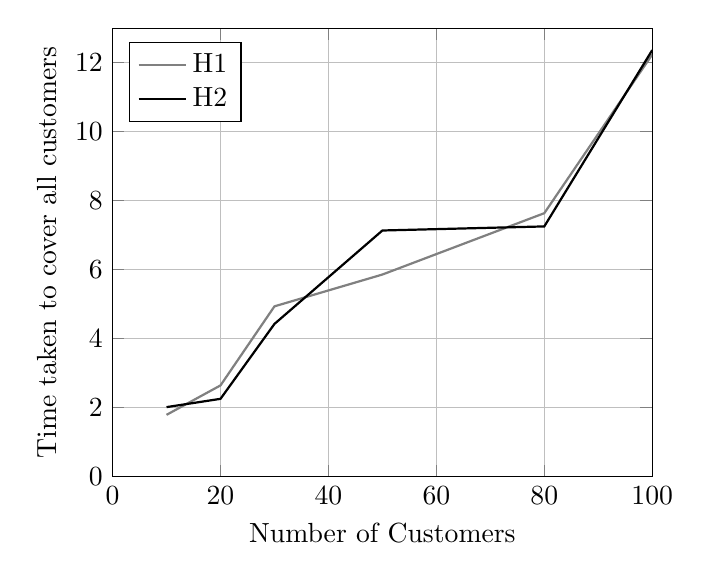
\begin{tikzpicture}
        \begin{axis}[
            xlabel={Number of Customers},
            ylabel={Time taken to cover all customers},
            xmin=0, xmax=100,
            ymin=0, ymax=13,
            grid=major,
            legend pos=north west
        ]
        
        \addplot[color=gray, thick] coordinates {
            (10, 1.78924)
            (20, 2.64235)
            (30, 4.93532)
            (50, 5.85753)
            (80, 7.636346)
            (100, 12.23632)
        };
        \addlegendentry{H1}
        
        \addplot[color=black, thick] coordinates {
            (10, 2.01293)
            (20, 2.25357)
            (30, 4.4252)
            (50, 7.13463)
            (80, 7.25263)
            (100, 12.36363)
        };
        \addlegendentry{H2}
        
        \end{axis}
    \end{tikzpicture}
    \caption{Graph of Heuristic1 and Heuristic2 Data with 40 charging and battery swapping stations and 15 vehicles(80-120kg)}
    \label{fig:h1-h2-graph}
\end{figure}


\begin{figure}
    \centering
    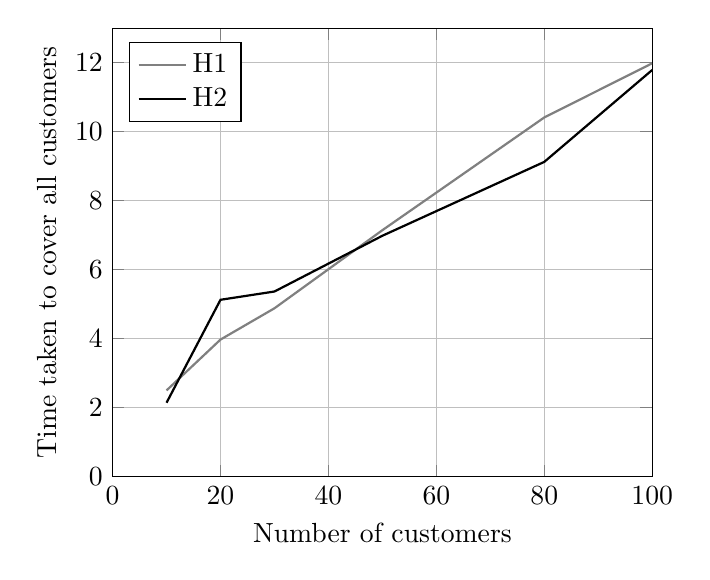
\begin{tikzpicture}
        \begin{axis}[
            xlabel={Number of customers},
            ylabel={Time taken to cover all customers},
            xmin=0, xmax=100,
            ymin=0, ymax=13,
            grid=major,
            legend pos=north west
        ]
        
        \addplot[color=gray, thick] coordinates {
            (10, 2.49702)
            (20, 3.97183)
            (30, 4.87913)
            (50, 7.143333)
            (80, 10.41242)
            (100, 11.98364)
        };
        \addlegendentry{H1}
        
        \addplot[color=black, thick] coordinates {
            (10, 2.14005)
            (20, 5.12538)
            (30, 5.36543)
            (50, 6.98242)
            (80, 9.124214)
            (100, 11.78934)
        };
        \addlegendentry{H2}
        
        \end{axis}
    \end{tikzpicture}
    \caption{Graph of Heuristic1 and Heuristic2 Data with 20 charging and battery swapping stations and 15 vehicles(80-120kg)}
    \label{fig:h1-h2-graph-updated}
\end{figure}


\section{Conclusion} \label{sec:CF}
In this work, we presented a framework that minimizes the
time in terms of maximum total time that a vehicle remains on a road with most optimum least cost. We have formulated the optimization problem as
MINLP, which finds an optimal solution. We proposed heuristic approaches for finding near-optimal solutions quickly. With the heuristic approach the problem can be solved for over 10000 nodes with hundreds of charging stations within seconds. The discussed problem can be
extended to optimize the performance with more reals world use cases like partial charging, dynamic delivery/pickup insertion, waiting time, and penalty costs.



\bibliographystyle{IEEEtran}
\bibliography{refr}





% that's all folks
\end{document}


